\documentclass[a4paper,14pt,oneside,final]{extarticle}
\usepackage[top=2cm, bottom=2cm, left=3cm, right=1cm]{geometry}
\usepackage{scrextend}

\usepackage[T2A,T1]{fontenc}
\usepackage[ukrainian,russian,english]{babel}
\usepackage{tempora}
\usepackage{fontspec}
\setmainfont{tempora}

% Зачем: Отключает использование изменяемых межсловных пробелов.
% Почему: Так не принято делать в текстах на русском языке.
\frenchspacing

\usepackage{indentfirst}
\setlength{\parindent}{1.25cm}
\renewcommand{\baselinestretch}{1.5}

% Header
\usepackage{fancyhdr}
\pagestyle{fancy}
\fancyhead{}
\fancyfoot{}
\fancyhead[R]{\small \selectfont \thepage}
\renewcommand{\headrulewidth}{0pt}

% Captions
\usepackage{chngcntr}
\counterwithin{figure}{section}
\counterwithin{table}{section}
\usepackage[tableposition=top]{caption}
\usepackage{subcaption}
\DeclareCaptionLabelFormat{gostfigure}{Рисунок #2}
\DeclareCaptionLabelFormat{gosttable}{Таблиця #2}
\DeclareCaptionLabelSeparator{gost}{~---~}
\captionsetup{labelsep=gost}
\captionsetup[figure]{labelformat=gostfigure}
\captionsetup[table]{labelformat=gosttable}
\renewcommand{\thesubfigure}{\asbuk{subfigure}}

% Sections
\usepackage[explicit]{titlesec}
\newcommand{\sectionbreak}{\clearpage}

\titleformat{\section}
  {\centering}{\thesection \quad}{0pt}{\MakeUppercase{#1}}
\titleformat{\subsection}[block]
  {\bfseries}{\thesubsection \quad #1}{0cm}{}

\titlespacing{\section} {0cm}{0cm}{21pt}
\titlespacing{\subsection} {\parindent}{21pt}{0cm}
\titlespacing{\subsubsection} {\parindent}{0cm}{0cm}

% Lists
\usepackage{enumitem}
\renewcommand\labelitemi{--}
\setlist[itemize]{noitemsep, topsep=0pt, wide}
\setlist[enumerate]{noitemsep, topsep=0pt, wide, label=\arabic*}
\setlist[description]{labelsep=0pt, noitemsep, topsep=0pt, leftmargin=2\parindent, labelindent=\parindent, labelwidth=\parindent, font=\normalfont}

% Toc
\usepackage{tocloft}
\tocloftpagestyle{fancy}
\renewcommand{\cfttoctitlefont}{}
\setlength{\cftbeforesecskip}{0pt}
\renewcommand{\cftsecfont}{}
\renewcommand{\cftsecpagefont}{}
\renewcommand{\cftsecleader}{\cftdotfill{\cftdotsep}}

\usepackage{float}
\usepackage{pgfplots}
\usepackage{graphicx}
\usepackage{multirow}
\usepackage{amssymb,amsfonts,amsmath,amsthm}
\usepackage{csquotes}

\usepackage{listings}
\lstset{basicstyle=\footnotesize\ttfamily,breaklines=true}
\lstset{language=Matlab}

\usepackage[
	backend=biber,
	sorting=none,
	language=auto,
	autolang=other
]{biblatex}
\DeclareFieldFormat{labelnumberwidth}{#1}

\lstdefinelanguage{Python}{
  keywords={and, break, class, continue, def, yield, del, elif, else, except, exec, finally, for, from, global, if, import, in, lambda, not, or, pass, print, raise, return, try, while, assert, with},
  keywordstyle=\color{NavyBlue}\bfseries,
  ndkeywords={True, False},
  ndkeywordstyle=\color{BurntOrange}\bfseries,
  emph={as},
  emphstyle={\color{OrangeRed}},
  identifierstyle=\color{black},
  sensitive=true,
  commentstyle=\color{gray}\ttfamily,
  comment=[l]{\#},
  morecomment=[s]{/*}{*/},
  stringstyle=\color{ForestGreen}\ttfamily,
  morestring=[b]',
  morestring=[s]{"""*}{*"""},
}


\usepackage{tabularx}
\usepackage{multicol}

\newcommand{\labnumber}{1} % first lab
\documentclass[a4paper,14pt,oneside,final]{extarticle}
\usepackage[top=2cm, bottom=2cm, left=3cm, right=1cm]{geometry}
\usepackage{scrextend}

\usepackage[T2A,T1]{fontenc}
\usepackage[ukrainian,russian,english]{babel}
\usepackage{tempora}
\usepackage{fontspec}
\setmainfont{tempora}

% Зачем: Отключает использование изменяемых межсловных пробелов.
% Почему: Так не принято делать в текстах на русском языке.
\frenchspacing

\usepackage{indentfirst}
\setlength{\parindent}{1.25cm}
\renewcommand{\baselinestretch}{1.5}

% Header
\usepackage{fancyhdr}
\pagestyle{fancy}
\fancyhead{}
\fancyfoot{}
\fancyhead[R]{\small \selectfont \thepage}
\renewcommand{\headrulewidth}{0pt}

% Captions
\usepackage{chngcntr}
\counterwithin{figure}{section}
\counterwithin{table}{section}
\usepackage[tableposition=top]{caption}
\usepackage{subcaption}
\DeclareCaptionLabelFormat{gostfigure}{Рисунок #2}
\DeclareCaptionLabelFormat{gosttable}{Таблиця #2}
\DeclareCaptionLabelSeparator{gost}{~---~}
\captionsetup{labelsep=gost}
\captionsetup[figure]{labelformat=gostfigure}
\captionsetup[table]{labelformat=gosttable}
\renewcommand{\thesubfigure}{\asbuk{subfigure}}

% Sections
\usepackage[explicit]{titlesec}
\newcommand{\sectionbreak}{\clearpage}

\titleformat{\section}
  {\centering}{\thesection \quad}{0pt}{\MakeUppercase{#1}}
\titleformat{\subsection}[block]
  {\bfseries}{\thesubsection \quad #1}{0cm}{}

\titlespacing{\section} {0cm}{0cm}{21pt}
\titlespacing{\subsection} {\parindent}{21pt}{0cm}
\titlespacing{\subsubsection} {\parindent}{0cm}{0cm}

% Lists
\usepackage{enumitem}
\renewcommand\labelitemi{--}
\setlist[itemize]{noitemsep, topsep=0pt, wide}
\setlist[enumerate]{noitemsep, topsep=0pt, wide, label=\arabic*}
\setlist[description]{labelsep=0pt, noitemsep, topsep=0pt, leftmargin=2\parindent, labelindent=\parindent, labelwidth=\parindent, font=\normalfont}

% Toc
\usepackage{tocloft}
\tocloftpagestyle{fancy}
\renewcommand{\cfttoctitlefont}{}
\setlength{\cftbeforesecskip}{0pt}
\renewcommand{\cftsecfont}{}
\renewcommand{\cftsecpagefont}{}
\renewcommand{\cftsecleader}{\cftdotfill{\cftdotsep}}

\newcommand{\khpistudentgroup}{КН-34г}
\newcommand{\khpistudentname}{Чепурний~А.~С.}

\newcommand{\khpidepartment}{Програмна інженерія та інформаційні технології управління}
\newcommand{\khpititlewhat}{
	Лабораторна робота №\labnumber \\
	з предмету <<Моделювання систем>>
}
\newcommand{\khpititlewho}{
	Виконав: \\
	\hspace*{\parindent} ст. групи \khpistudentgroup \\
	\hspace*{\parindent} \khpistudentname \\
	Перевірила: \\
	\hspace*{\parindent} ст. в. каф. ПІІТУ \\
	\hspace*{\parindent} Єршова~С.~І. \\
	\hspace*{\parindent} ас. каф. ПІІТУ \\
	\hspace*{\parindent} Литвинова~Ю.~С. \\
}



\graphicspath{{figures/}}

\begin{document}
\Ukrainian

\begin{titlepage}

\begin{center}
	МІНІСТЕРСТВО ОСВІТИ І НАУКИ УКРАЇНИ \\
	НАЦІОНАЛЬНИЙ ТЕХНІЧНИЙ УНІВЕРСИТЕТ \\
	«ХАРКІВСЬКИЙ ПОЛІТЕХНІЧНИЙ ІНСТИТУТ» \\[0.5cm]
	Кафедра <<\khpidepartment>> \\
\end{center}

\vspace{6cm}

\begin{center}
	\khpititlewhat
\end{center}

\vspace{3cm}

\begin{addmargin}[10cm]{0cm}
	\khpititlewho
\end{addmargin}

\vspace{\fill}

\begin{center}
	Харків \the\year
\end{center}

\end{titlepage}

\addtocounter{page}{1}

\section{ЭЛЕМЕНТЫ КЛАСТЕРА HADOOP}
\subsection*{Цель}
Исследование кластера Hadoop.
\subsection*{Задачи}
\begin{itemize}
    \item выявить преимущества и недостатки Hadoop;
    \item проанализировать структуру и основные этапы внедрения Hadoop;
    \item исследовать основные возможности Hadoop.
\end{itemize}

\subsection{Преимущества и недостатки Hadoop}
Преимущества Hadoop:
\begin{enumerate}
    \item Разнообразные источники данных.
    \item Эффективное хранение данных.
    \item Высокая производительность.
    \item Высокая отказоустойчивость.
    \item Низкий сетевой трафик.
    \item Открытый исходный код.
    \item Масштабируемость.
    \item Легкость использования.
    \item Совместимость.
    \item Поддержка множества языков программирования.
\end{enumerate}

Недостатки Hadoop:
\begin{enumerate}
    \item Размер блока в файловой системе не может быть меньше 128 мегабайт.
    \item Невозможность произведения вычислений в памяти.
    \item Невозможность работы в интерактивном режиме обработки данных.
    \item Сложность защиты данных.
\end{enumerate}

\subsection{Компоненты экосистемы Hadoop}
Компоненты экосистемы Hadoop представлены на рисунке~\ref{fig:hadoop_ecosystem}.

\begin{figure}[H]
    \centering
    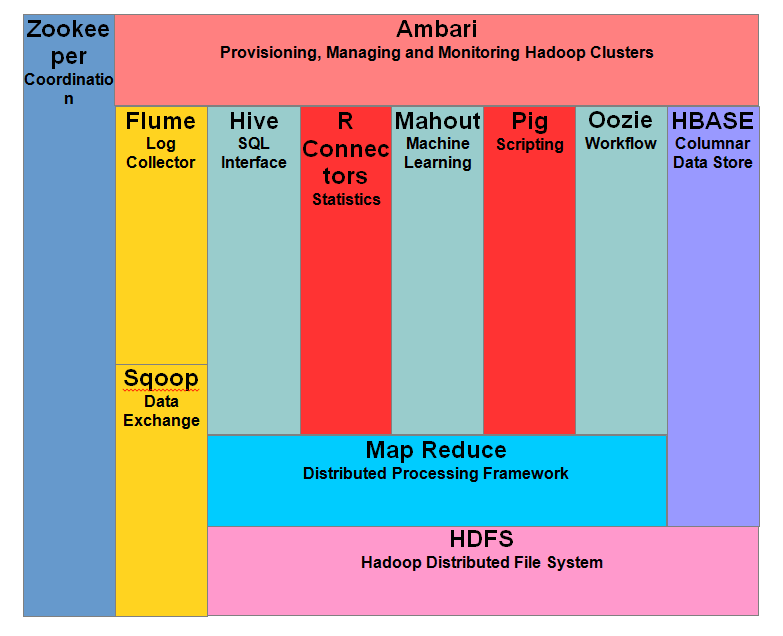
\includegraphics[width=0.6\textwidth]{hadoop_ecosystem}
    \caption{Компоненты Hadoop}
    \label{fig:hadoop_ecosystem}
\end{figure}

\begin{itemize}
    \item Hadoop MapReduce -- вычислительная модель и фреймворк для распределенной обработки большого количества данных.

          \begin{tabularx}{450pt}{X|X}
              \textbf{Преимущества}     & \textbf{Недостатки} \\
              \hline
              \begin{itemize}[noitemsep,nolistsep,leftmargin=0pt,labelindent=0pt]
                  \item поддержка библиотек разработанных для JVM;
                  \item платформонезависимость.
              \end{itemize} &
              \begin{itemize}[noitemsep,nolistsep,leftmargin=0pt,labelindent=0pt]
                  \item неприменимо для интерактивного анализа.
              \end{itemize}
          \end{tabularx}\\
    \item HDFS (Hadoop Distributed File System) -- файловая система.

          \begin{tabularx}{450pt}{X|X}
              \textbf{Преимущества}     & \textbf{Недостатки} \\
              \hline
              \begin{itemize}[noitemsep,nolistsep,leftmargin=0pt,labelindent=0pt]
                  \item высокая пропускная способность;
                  \item отказоустойчивость.
              \end{itemize} &
              \begin{itemize}[noitemsep,nolistsep,leftmargin=0pt,labelindent=0pt]
                  \item операция слияния данных с множества баз данных медленная и тяжело реализуемая.
              \end{itemize}
          \end{tabularx}\\
    \item YARN -- автоматический планировщик ресурсов кластера.
    \item HBase -- это распределенная, колоночно-ориентированная, мультиверсионная база типа <<ключ-значение>>.
    \item Zookeeper -- сервис, который предназначен для некой координации взаимодействия процессов в распределенных системах, в распределенных приложениях.
    \item Ambari -- сервис, нацеленный на упрощение работы с Hadoop при помощи разработанного программного обеспечения для управления и контроля кластеров.
    \item Flume -- инструмент, позволяющий управлять потоками данных и, в конечном счете, передавать их на некоторый <<пункт назначения>>.
    \item Sqoop -- инструмент, предназначенный для передачи данных между Hadoop и реляционными базами данных или мэйнфреймами.
    \item Hive -- система управления базами данных на основе платформы Hadoop.
    \item Mahout -- библиотека для машинного обучения.
    \item R connectors -- позволяет писать mapreduce на R.
\end{itemize}

\subsection{Этапы внедрения Hadoop}
Перед интеграцией Hadoop необходимо выполнить следующие этапы:
\begin{enumerate}
    \item Хранение данных: архивация, хранение информации в файлах, масштабируемость, репликация, обработка отказов;
    \item Чтение данных: разархивация, распараллеливание, SQL доступ;
    \item Сбор данных.
    \item Подготовка данных: построение ROLAP/MOLAP моделей, ETL.
\end{enumerate}

\subsection{Применение Hadoop}
Hadoop следует применять для решение таких проблем:
\begin{enumerate}
    \item Обработка большого количества данных (ТБ или выше).
    \item Надежное хранение разнообразных данных.
    \item Параллельная обработка данных.
\end{enumerate}

\subsection*{Выводы}
В процессе выполнения лабораторной работы было выявлены преимущества и недостатки Hadoop, определены типы проблем решаемых с помощью Hadoop, описаны главные компоненты системы.

Hadoop следует использовать для параллельной обработки большого количества данных.

\end{document}
